\documentclass[12pt,letterpaper]{article}
\usepackage[top=2cm, bottom=4.5cm, left=2.5cm, right=2.5cm]{geometry}
\usepackage{fancyhdr}
\usepackage{amsmath}
\usepackage{graphicx}
\usepackage{float}
\setlength{\parindent}{0.0in}
\setlength{\parskip}{0.05in}

\newcommand\course{CSE 417T}
\newcommand\hwnumber{4}                  % <-- homework number
\newcommand\Name{Isabelle Xu and Clayton Knittel}         


\pagestyle{fancyplain}
\headheight 35pt
\lhead{\Name}
\chead{\textbf{\Large Homework \hwnumber}}
\rhead{\course \\ \today}
\lfoot{}
\cfoot{}
\rfoot{\small\thepage}
\headsep 1.5em

\begin{document}

\section*{Problem 1}

\begin{description}
	\item (a) \& (b)

\begin{figure}[H]
\centering
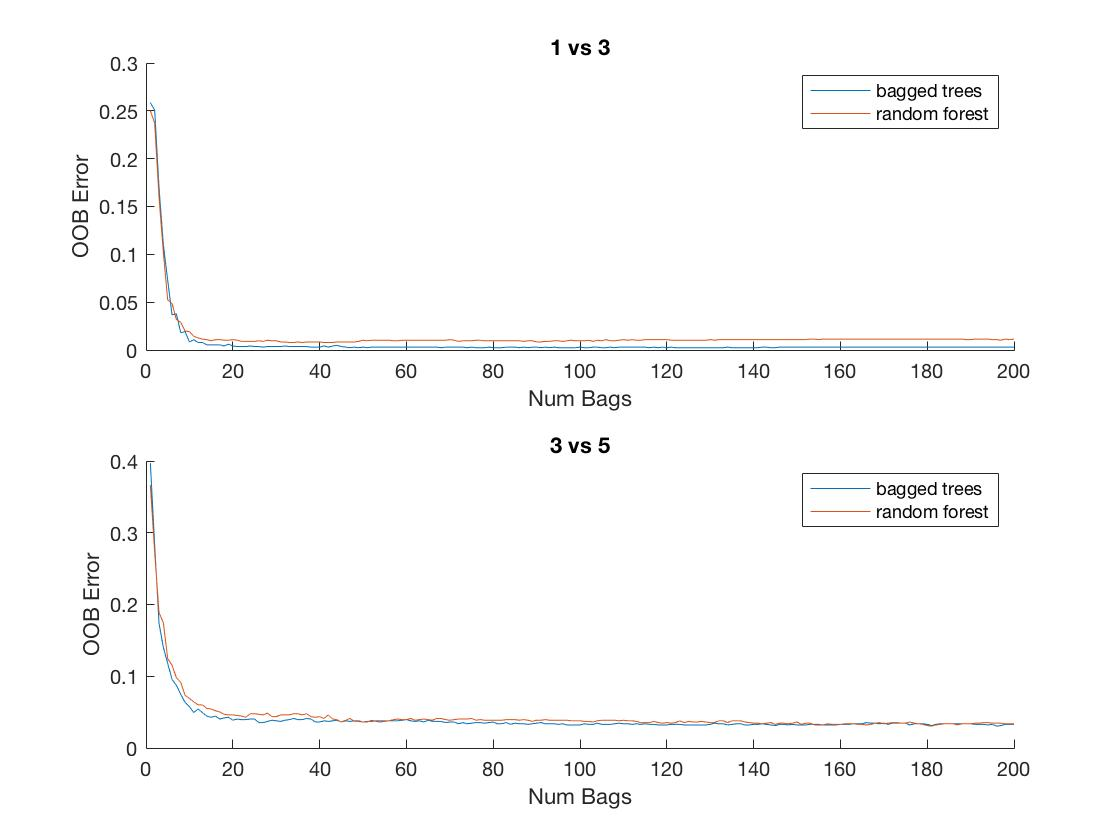
\includegraphics[scale=0.28]{image.jpg} 
\end{figure}

	\item (c)

\end{description}

\end{document}